% !TeX spellcheck = en_US
\section*{Long-run of RNN-MSNN}

Test report

by E. Marquer, 2018/05/29, Synalp and Université de Lorraine

\subsection{Abstract}

The run was done on the reduced enwik8 corpus.

The test is composed of 4 successive runs:
\begin{itemize}
	\item 1 run of 2h on grimani-4;
	\item 2 runs of 12h, both on grimani-1;
	\item 1 run of 50h on grele-11;
\end{itemize}

End causes are as follow: 
\begin{itemize}
	\item Run 1: out of time (2h);
	\item Run 2: out of time (12h);
	\item Run 3: end of epoch crash (7h30);
	\item Run 4: end of epoch crash (19h15);
\end{itemize}

Mean time for an epoch is about 19h 15min (on the reduced version of the
corpus). Two epochs were completed.

\subsection{Results}

Each run crashed between epochs, so a bit of patching had to be made on
top of fixing the bug.

\subsubsection{Memory}

Both RAM and video RAM are still subject to a constant leak in memory.
But even if it does not show on the plots (scale is too small), logs
confirm that there is no leak during validation.

\begin{figure}[H]
\centering
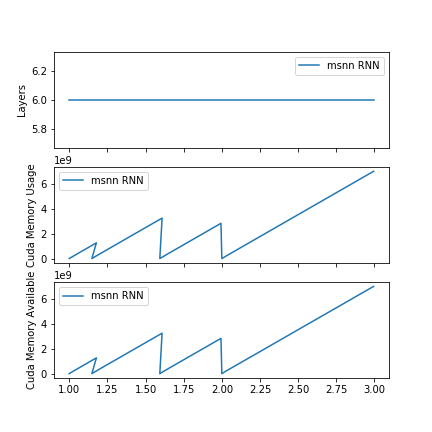
\includegraphics{parts/appendix/reports-gmsnn/docs_esteban-latex/test_reports/2018-06-11/memory.png}
\caption{Memory usage}
\end{figure}

\begin{figure}[H]
\centering
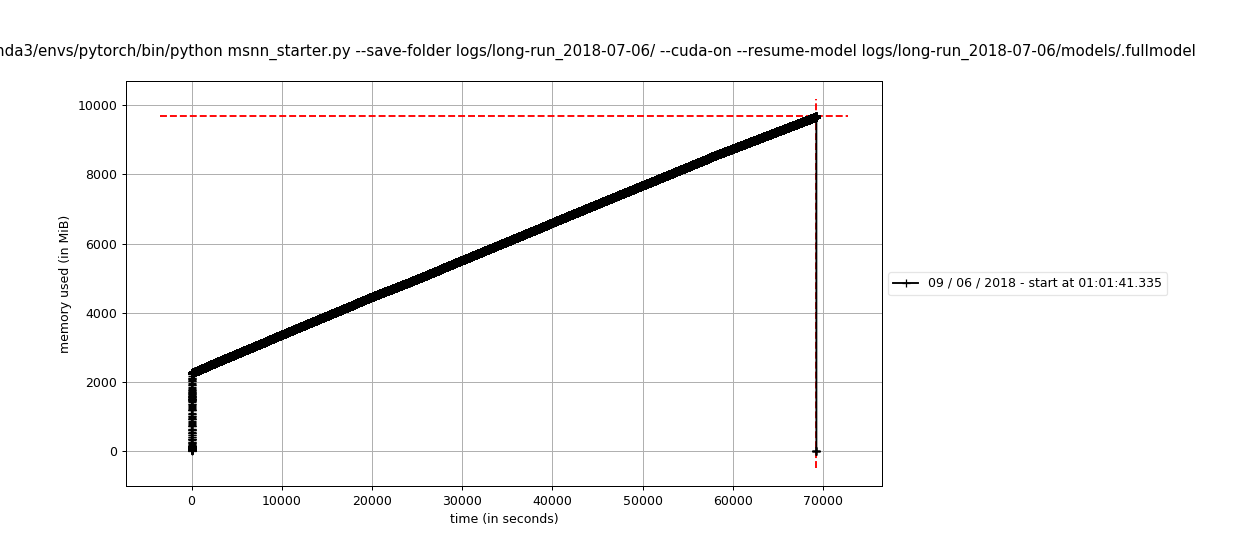
\includegraphics[width=\textwidth]{parts/appendix/reports-gmsnn/docs_esteban-latex/test_reports/2018-06-11/RAM_restart-2.png}
\caption{RAM third run}
\end{figure}

An other noticeable property is that ``Run Time'', corresponding to the
time to train over \emph{log\_interval} sequences, is mostly
proportional to CUDA memory usage. The source of the cuda memory leak is
probably the same as what makes training slower.

\begin{figure}[H]
\centering
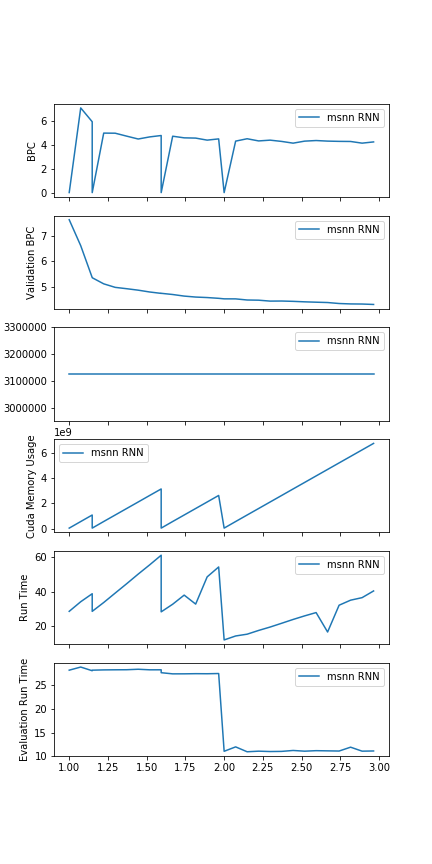
\includegraphics[height=.8\textheight]{parts/appendix/reports-gmsnn/docs_esteban-latex/test_reports/2018-06-11/frac.png}
\caption{Memory and computation time}
\end{figure}

\newpage
\subsubsection{BPC / Validation BPC}

BPC and Validation BPC

\begin{figure}[H]
\centering
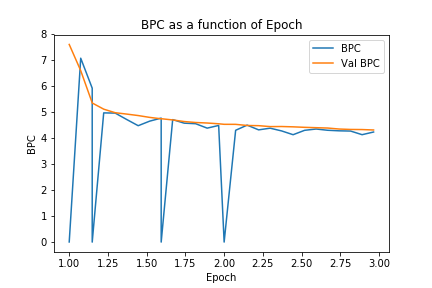
\includegraphics[width=\textwidth]{parts/appendix/reports-gmsnn/docs_esteban-latex/test_reports/2018-06-11/frac_val_bpc.png}
\caption{BPC}
\end{figure}


\newpage
\subsubsection{Job restart}\label{job-restart}

When resuming a job, CUDA memory is entirely freed. Same thing can be
said about RAM.

\begin{figure}[H]
\centering
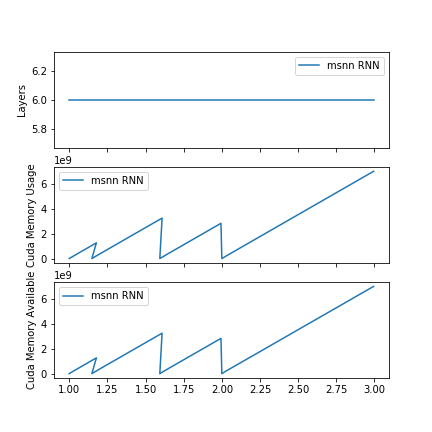
\includegraphics[width=\textwidth]{parts/appendix/reports-gmsnn/docs_esteban-latex/test_reports/2018-06-11/memory.png}
\caption{Memory usage}
\end{figure}

\begin{figure}[H]
\centering
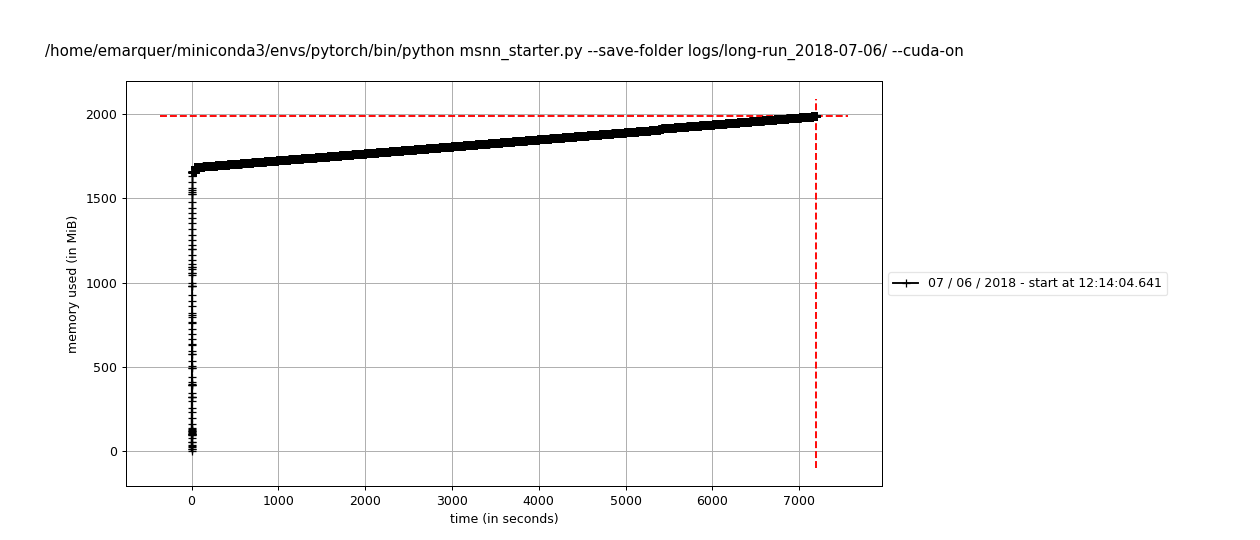
\includegraphics[width=\textwidth]{parts/appendix/reports-gmsnn/docs_esteban-latex/test_reports/2018-06-11/RAM.png}
\caption{RAM first run}
\end{figure}

\begin{figure}[H]
\centering
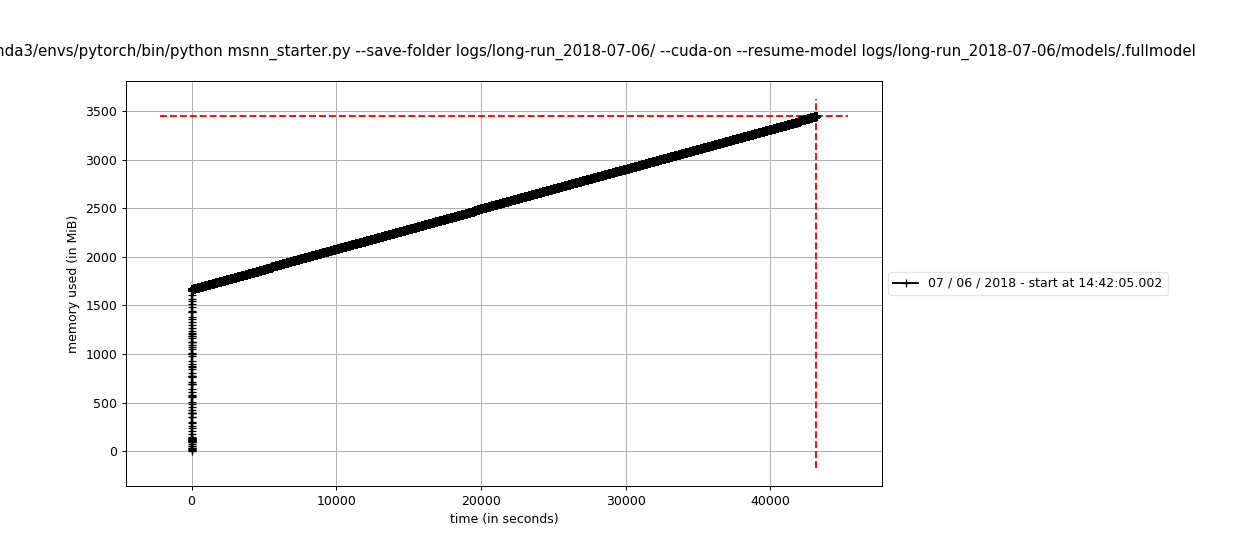
\includegraphics[width=\textwidth]{parts/appendix/reports-gmsnn/docs_esteban-latex/test_reports/2018-06-11/RAM_restart-1.png}
\caption{RAM second run}
\end{figure}

\begin{figure}[H]
\centering
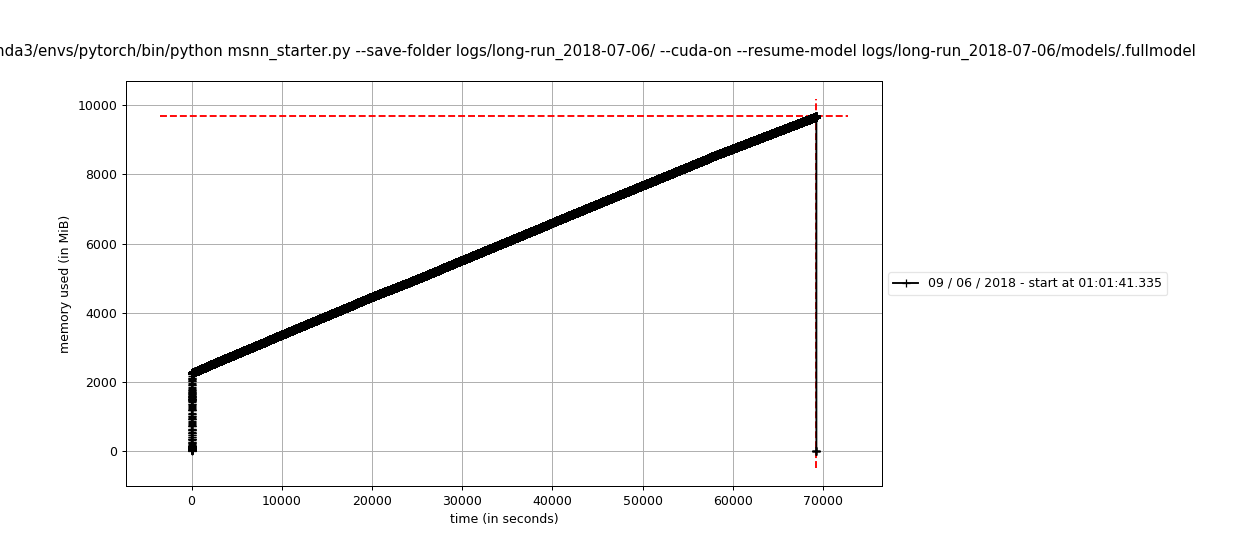
\includegraphics[width=\textwidth]{parts/appendix/reports-gmsnn/docs_esteban-latex/test_reports/2018-06-11/RAM_restart-2.png}
\caption{RAM third run}
\end{figure}

Memory is freed each time the job is restarted, meaning either a part of
the necessary is discarded, or unnecessary data is kept in memory. As in
CUDAles tests a memory maximum was reached, CUDA seems to be the source
of the leak (data copies not removed, \ldots{}).

\subsection{Next steps}

Debug end of epoch bug. Try to patch memory leak. Continue training.
